In the previous sections, we have detailed the path solver, which computes propagation paths and the related electric fields from a source to a target. Now, we turn our attention to the radio map solver, which computes a \emph{radio map} (also known as \emph{coverage map} or \emph{power map}) for a given scene and source. While we describe the algorithm for a single source, \SRT{} can compute radio maps for multiple sources in parallel.

\begin{figure}[ht!]
    \centering
    \begin{subfigure}[b]{0.6\textwidth}
        \centering
        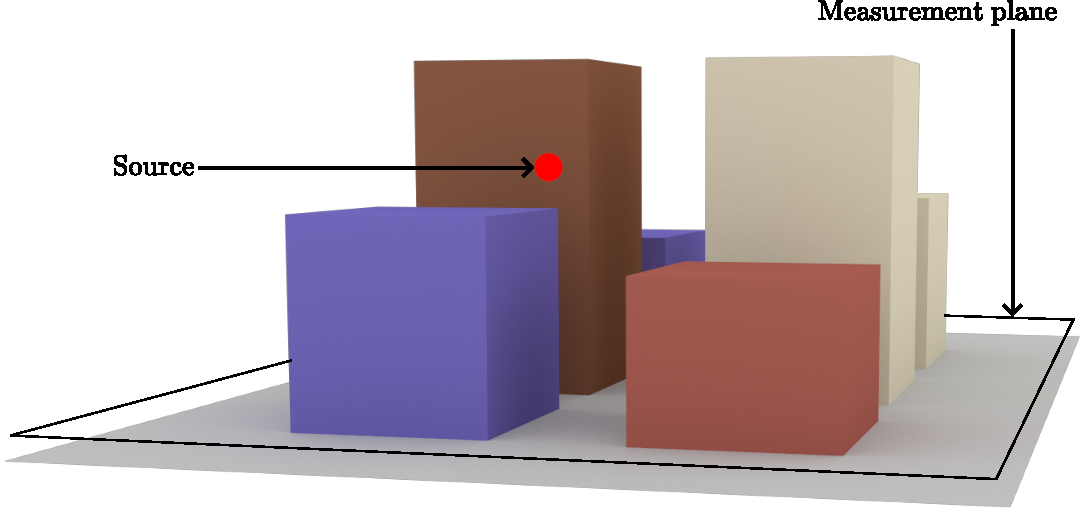
\includegraphics[width=\textwidth]{figures/radio-map-solver-eg-a.pdf}
        \caption{Scene with a measurement plane.}
    \end{subfigure}

    \begin{subfigure}[b]{0.6\textwidth}
        \centering
        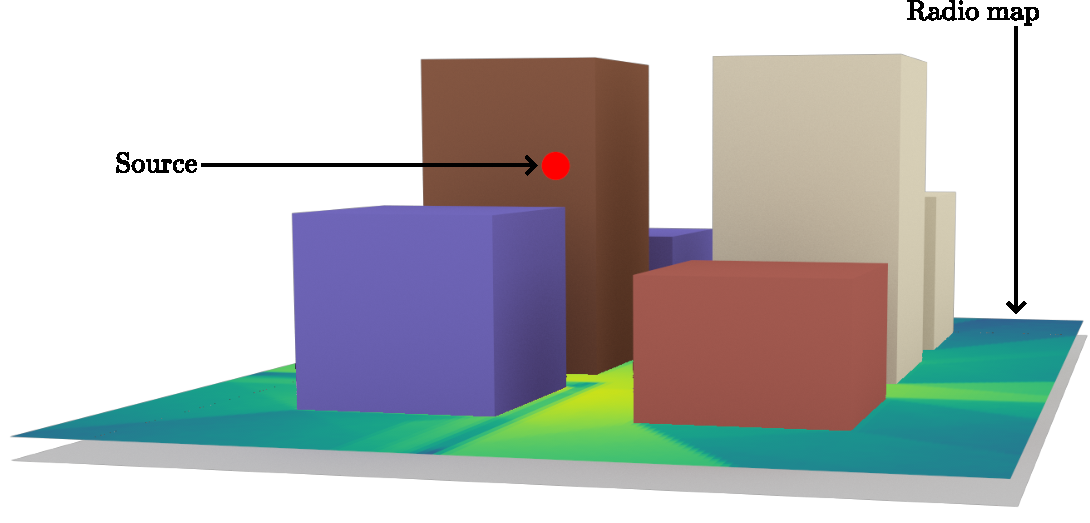
\includegraphics[width=\textwidth]{figures/radio-map-solver-eg-b.pdf}
        \caption{Radio map for the measurement plane in (a).}
    \end{subfigure}
    \caption{(a) A measurement surface, which is here a plane parallel to the ground, is placed in the scene to capture paths without affecting their propagation, (b) the resulting radio map showing the spatial distribution of channel gains.\label{fig:radio-map-solver-eg}}
\end{figure}

A radio map estimates the channel gain~\eqref{eq:channel-gain} from a source to each point on a \emph{measurement surface}, as illustrated in Figure~\ref{fig:radio-map-solver-eg}. The measurement surface is partitioned into \emph{measurement cells}, which are assumed to be planar. For each cell, the solver estimates the average channel gain that would be observed by a target placed within that cell.
Note that the measurement surface does not interact with the electromagnetic waves, but only serves to capture the paths that intersect it.
Moreover, a ray can intersect the measurement surface at multiple points.

In Section~\ref{sec:radio-map-solver-definition}, we present a definition of radio maps that allows for their efficient computation using \gls{SBR}. This approach makes the computation of radio maps both fast and scalable.

\subsection{Definition of Radio Map}
\label{sec:radio-map-solver-definition}

We define radio maps as path integrals, similar to how measurements are defined in computer graphics~\cite[Section~3.7]{10.1145/15886.15902,
Veach:1997:RMC}.
Consider a point source $\sv$. The measurement surface, denoted by $\Mc$, is divided into $N_M$ cells $M_i$, for $i = 1, \dots, N_M$, each of area $\abs{M_i}$.
Ignoring diffraction for now, let $\Ac$ denote the union of all scatterer surfaces in the scene. We define
\begin{equation}
    \Ac^{\ell} = \underbrace{\Ac \times \cdots \times \Ac}_{\ell\text{ times}}
\end{equation}
as the set of all sequences of $\ell$ vertices representing interactions with scatterers surfaces—that is, all paths of length $\ell$ that are not diffracted,
\begin{equation}
    p = \LB \vv^{(1)}, \cdots, \vv^{(\ell)} \RB.
\end{equation}
A path from $\sv$ to a point $\tv \in \Mc$ can be written as $\LB \sv, p, \tv\RB$, though for brevity we refer simply to the path $p$.
Note that $\Ac^{0}$ corresponds to the \gls{LoS} path from $\sv$ to $\tv$.

Focusing on paths of a fixed length $\ell$, we define the radio map value for the $i$-th cell as follows:
\begin{equation}
    \label{eq:radio-map-solver-ci-ell}
    C_i^{(\ell)} = \frac{1}{\abs{M_i}} \int_{M_i} \int_{\Ac^{\ell}} e \LB p \RB \Vc\LB p \RB w \LB p \RB\, d\mu^{(\ell)}(p)\, d\tv
\end{equation}
where $d\tv$ is an infinitesimal surface element on the measurement surface $M_i$, and $\mu^{(\ell)}(p)$ is the area-product measure on the scattering surface, i.e.,
\begin{equation}
    d\mu^{(\ell)}(p) = dA(\vv^{(1)}) \dots dA(\vv^{(\ell)}).
\end{equation}
$\Vc\LB p \RB$ is the indicator function which equals to $1$ if the path is not occluded and $0$ otherwise, and $e(p)$ is the channel gain for the path, defined as
\begin{equation}
    \label{eq:radio-map-solver-path-gain}
    e(p) = \norm{ \frac{\lambda}{4\pi}  \Tm \Cm_\text{T}(\theta_\text{T}, \varphi_\text{T})  }^2.
\end{equation}
Here, $\lambda$ is the wavelength, $\Cm_\text{T}$ is the $2$-dimensional complex vector of the transmit antenna pattern evaluated at the departure angles $(\theta_\text{T}, \varphi_\text{T})$ of $p$, and $\mathbf{T}$ is a $2 \times 2$ complex matrix modeling the effects of scatterers and free-space path loss along $p$. Unlike in~\eqref{eq:path-coefficient}, the receive antenna pattern is not applied; instead, the squared norm of the electric field is used. This corresponds to assuming a receiver equipped with an isotropic antenna whose polarization is matched to the one of the incident wave.
Note that since $e(p)$ is the squared norm of the electric field amplitude, the radio map represents a non-coherent sum of the path gains.

In~\eqref{eq:radio-map-solver-ci-ell}, $w(p)$ restricts which paths are considered:
\begin{equation}
    \label{eq:radio-map-solver-w}
    w(p) = \prod_{i=1}^{\ell} w^{(i)}(\widehat{\kv}_i^{(i)}, \widehat{\kv}_s^{(i)}),
\end{equation}
where $\widehat{\kv}_i^{(i)}$ is the incident wave direction at the $i$-th interaction, $\widehat{\kv}_s^{(i)}$ is the scattered wave direction at the $i$-th interaction, and $w^{(i)}$ depends on the types of interactions considered for the $i$-th interaction. For instance, if only specular reflections and refractions are allowed at the $i$-th interaction,
\begin{equation}
    \label{eq:radio-map-solver-w-refl-refr}
    w^{(i)}(\widehat{\kv}_i^{(i)}, \widehat{\kv}_s^{(i)}) =
    \underbrace{\delta \LB \widehat{\kv}_s^{(i)} - \frac{\widehat{\kv}_i^{(i)} - 2\LB \widehat{\nv}\tp\widehat{\kv}_i^{(i)} \RB \widehat{\nv}_s^{(i)}}{\norm{\widehat{\kv}_i^{(i)} - 2\LB \widehat{\nv}\tp\widehat{\kv}_i^{(i)} \RB \widehat{\nv}_s^{(i)}}} \RB}_{\text{Specular reflection}}
    +
    \underbrace{\delta \LB \widehat{\kv}_s^{(i)} - \widehat{\kv}_i^{(i)} \RB}_{\text{Refraction}}
\end{equation}
where $\widehat{\nv}$ is the normal to the scatterer's surface.
Although $w(p)$ could in principle be absorbed into $e(p)$, as usually done in the computer graphics literature, we keep it separate for clarity.

The overall radio map value for the $i$-th cell is given by summing over all possible path depths $\ell = 0, 1, \ldots, \infty$:
\begin{equation}
    \label{eq:radio-map-solver-ci-all}
    C_i = \sum_{\ell=0}^{\infty} C_i^{(\ell)}
        = \frac{1}{\abs{M_i}} \int_{M_i} \sum_{\ell=0}^{\infty} \int_{\Ac^{\ell}} e \LB p \RB \Vc\LB p \RB w \LB p \RB\ d\mu^{(\ell)}(p) d\tv.
\end{equation}

\begin{highlightbox}{Relation to computer graphics}
    Defining radio maps as path integrals closely parallels the measurement equation used in computer graphics (see, e.g.,~\cite[Eq.~3.18]{Veach:1997:RMC}).
    Specifically, following~\cite[Chapter~8]{Veach:1997:RMC}, the radio map definition~\eqref{eq:radio-map-solver-ci-all} can be rewritten as:
    \begin{equation}
        \label{eq:radio-map-solver-ci-all-integral}
        C_i = \frac{1}{\abs{M_i}} \int_{M_i} \int_{\Ac^{\infty}} e \LB p \RB \Vc\LB p \RB w \LB p \RB\ d\mu(p) d\tv,
    \end{equation}
    where
    \begin{align}
        \Ac^{\infty} &= \bigcup_{\ell=0}^{\infty} \Ac^{\ell}, \label{eq:radio-map-solver-Ac-infty}\\
        \mu(P) &= \sum_{\ell=0}^{\infty} \mu^{(\ell)}\LB P \cap \Ac^{\ell} \RB \label{eq:radio-map-solver-mu-P}
    \end{align}
    where $P \subset \Ac^{\infty}$ is any set of paths.
    Intuitively, by defining~\eqref{eq:radio-map-solver-Ac-infty} and~\eqref{eq:radio-map-solver-mu-P}, the infinite sum over path depths in~\eqref{eq:radio-map-solver-ci-all} can be replaced with the integral in~\eqref{eq:radio-map-solver-ci-all-integral}. This provides a path integral formulation for the radio map, analogous to~\cite[Eq.~8.5]{Veach:1997:RMC}. This analogy enables the use of computer graphics techniques for radio map computation, including methods for improving sample efficiency.

    It is important to note that this analogy does not extend to the path solver, which is not concerned with evaluating an integral but rather with finding a set of paths, which are not aggregated into a single scalar value. However, if the objective is limited to calculating channel tap coefficients, then a similar analogy can be made.
    Considering a target $\tv$, the definition of a channel tap coefficient~~\cite[Eq.~2.36]{Tse} can be rewritten as:
    \begin{equation}
        h_i = \int_{\Ac^{\infty}} a(p) \Vc\LB p \RB w(p) \text{sinc}\LB i  - \frac{\tau(p)}{T_s} \RB d\mu(p)
    \end{equation}
    where, $i \in \ZZ$ denotes the tap index, $a(p)$ is the complex-valued path coefficient~\eqref{eq:path-coefficient}, $\tau(p)$ the propagation delay, and $T_s$ the sampling period.
    Note that, as previously mentioned, $p$ is a shorthand for the path $\LB \sv, p, \tv\RB$.
    Unlike~\cite[Eq.~2.36]{Tse}, an integral is used (instead of a sum) to account for the continuous set of propagation directions. In this equation, each tap coefficient can be interpreted as a measurement. However, in contrast to computer graphics and radio map computations—which involve a non-coherent sum of amplitude magnitudes—the tap coefficients involve a coherent aggregation of the path contributions, since the complex-valued $a(p)$ is used rather than only its amplitude. The same analogy applies to the channel frequency response (see, e.g.,~\cite[Eq.~3.138]{Tse}), for which each frequency bin is likewise treated as a measurement.
\end{highlightbox}

While the definition~\eqref{eq:radio-map-solver-ci-all} is comprehensive, it is not practical for computation as-is.
Indeed, directly integrating over the surfaces of the measurement cells would require connecting points on the measurement surface to the source, for example by placing one or more targets within each cell and using the path solver to compute the connecting paths. However, because accurately computing fine-grained radio maps typically demands a large number of target points, this approach is computationally prohibitive.
Instead, we use Monte Carlo integration with a single \gls{SBR} loop to efficiently estimate the value of each cell.
However, \gls{SBR} is not applicable to paths that include diffraction: as explained in Section~\ref{sec:path-solver-sbr}, the probability of a ray intersecting an edge is zero.
To address this, \SRT{} computes the radio map in two steps, as illustrated in Figure~\ref{fig:radio-map-solver-steps}.
First, the radio map is computed for all interaction types except diffraction using a single \gls{SBR} loop; wedges near the source are detected and stored during this step.
Second, only diffracted paths are computed.
Currently, \SRT{} supports only first-order diffraction for radio map computation, i.e., paths connecting the source to the measurement surface through a single diffracting wedge.
The two radio maps are then summed to obtain the final result.
The following describes the computation for each step.

\begin{figure}[ht!]
    \centering
    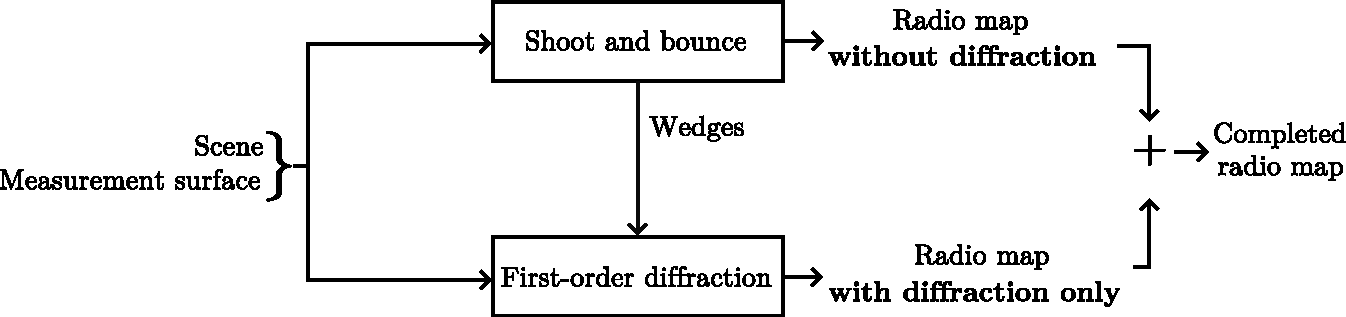
\includegraphics[width=0.85\textwidth]{figures/radio-map-solver-steps.pdf}
    \caption{Computation of the radio map in two steps: first, the radio map is computed for all interaction types except diffraction using a single \gls{SBR} loop; second, only diffracted paths are computed. The two radio maps are then summed to obtain the final radio map.\label{fig:radio-map-solver-steps}}
\end{figure}

\subsection{Computation of Radio Map without Diffraction}
\label{sec:radio-map-solver-sbr}

When diffraction is ignored, the radio map can be efficiently computed using a single \gls{SBR} loop. This is achieved by reformulating the radio map definition~\eqref{eq:radio-map-solver-ci-all} so that the integration is performed over the directions of rays originating from points that spawn ray tubes intersecting the measurement surface, rather than directly over the measurement surface itself. This is enabled by applying the change of variables $d\tv = \frac{r^2}{\cos \theta} d\omega$, where $r$ is the length of the ray tube on the measurement surface, $\theta$ is the angle between the incident ray and the normal of the measurement surface, and $d\omega$ is the infinitesimal solid angle subtended by the ray tube (see Section~\ref{sec:essential-concepts-ray-tube}). Thus, $d\tv$ represents the intersection area of the ray tube on the measurement surface.
With this change of variables, the radio map definition~\eqref{eq:radio-map-solver-ci-all} can be rewritten as:
\begin{equation}
    \label{eq:radio-map-solver-ci-all-2}
    C_i = \frac{1}{\abs{M_i}} \sum_{\ell=0}^{\infty} \int_{\Ac^{\ell}} \int_{\Omega} e \LB p \RB \Vc\LB p \RB w(p) \frac{r^2}{\cos \theta} d\omega d\mu^{(\ell)}(p).
\end{equation}
where $\Omega$ is the set of all directions of rays originating from points that spawn ray tubes intersecting the measurement surface, typically a hemisphere or a sphere.

Expression~\eqref{eq:radio-map-solver-ci-all-2} can be estimated as follows. Paths are generated by launching $N_S$ rays from the source $\sv$ and tracing their interactions with the scene geometry, thus performing a Monte Carlo integration over the surfaces of the scatterers $\Ac$. Intuitively, when a ray intersects a scatterer surface, it samples a surface element $\Delta A$ that corresponds to the ray tube intersection area, given by $\Delta A = \frac{r^2}{\cos \theta} \Delta \omega$, where $r$ denotes the ray tube length, $\theta$ is the angle between the incident ray and the surface normal, and $\Delta \omega$ is the solid angle subtended by the ray tube. The maximum path depth is set to $L < \infty$, and since a single path may intersect the measurement surface at multiple depths, all path depths $\ell = 0, 1, \ldots, L$ are considered. Interaction types (specular reflection, refraction, or diffuse reflection) are sampled according to~\eqref{eq:path-solver-used-dist-event}.

\begin{figure}[ht!]
    \centering
    \begin{subfigure}[b]{0.20\textwidth}
        \centering
        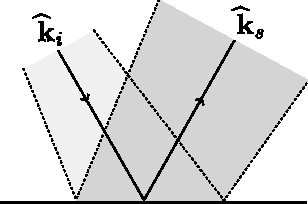
\includegraphics[width=\textwidth]{figures/radio-map-solver-ray-tubes-spec.pdf}
        \caption{Specular reflection}
        \label{fig:radio-map-solver-sbr-1}
    \end{subfigure}%
    \hspace{7em}
    \begin{subfigure}[b]{0.20\textwidth}
        \centering
        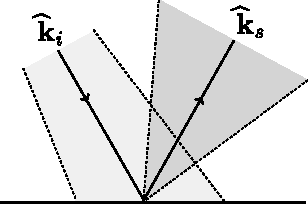
\includegraphics[width=\textwidth]{figures/radio-map-solver-ray-tubes-diff.pdf}
        \caption{Diffuse reflection}
        \label{fig:radio-map-solver-sbr-2}
    \end{subfigure}
    \caption{A specular reflection (left) deviates the incident ray tube, while a diffuse reflection (right) spawns a new ray tube. Shown in 2D for clarity.\label{fig:radio-map-solver-sbr}}
\end{figure}

This process leads to the following Monte Carlo estimator for the radio map~\eqref{eq:radio-map-solver-ci-all-2}:
\begin{equation}
    \label{eq:radio-map-solver-ci-all-2-estimator}
    \widehat{C}_i = \frac{1}{\abs{M_i}} \sum_{n=1}^{N_S} \sum_{\ell = 0}^L e \LB p_n^{(\ell)} \RB \mathbb{I}\LB p_n^{(\ell)} \RB \frac{\beta_n^{(\ell)}}{\Pr \LB \boldsymbol{\chi}_n^{(\ell)} \RB},
\end{equation}
where $p_n^{(\ell)}$ denotes the $n$-th path at depth $\ell$; $\mathbb{I}\LB p_n^{(\ell)} \RB$ is an indicator function equal to $1$ if $p_n^{(\ell)}$ intersects the measurement surface at depth $\ell$ and $0$ otherwise; and $\Pr \LB \boldsymbol{\chi}_n^{(\ell)} \RB$ is the probability of sampling the specific sequence of interaction types $\boldsymbol{\chi}_n^{(\ell)}$ corresponding to $p_n^{(\ell)}$.
$\beta_n^{(\ell)}$ is a weighting factor that incorporates the intersection area of the ray tubes on the scatterer and measurement surfaces, and thus absorbs the factor $\frac{r^2}{\cos \theta}$,
\begin{equation}
    \beta_n^{(\ell)} = \prod_{i=1}^{n_{\text{rt}}} \frac{r_i^2}{\cos \theta_i} \Delta\omega_i,
\end{equation}
where, for the $n$-th path at depth $\ell$, $n_{\text{rt}}$ is the number of ray tubes that constitute the path, $r_i$ is the length of the $i$-th ray tube, $\theta_i$ is the angle between the incident ray tube and the surface normal, and $\Delta\omega_i$ is the solid angle subtended by the $i$-th ray tube.
In the current propagation model of \SRT{}, only the source $\sv$ and diffuse reflection points act as point sources that spawn new ray tubes, whereas specular reflection and refraction points merely deviate existing ray tubes rather than spawning new ones. This is illustrated in Figure~\ref{fig:radio-map-solver-sbr}. The source emits $N_S$ ray tubes, each subtending a solid angle of $\frac{4\pi}{N_S}$, while each diffuse reflection point spawns a single ray tube, uniformly sampled over the hemisphere, with a solid angle of $2\pi$. Thus, $n_{\text{rt}}$ equals the number of diffuse reflection points along the path plus one.

\subsection{Computation of Radio Map due to Diffraction}
\label{sec:radio-map-solver-diffraction}

The \SRT{} radio map solver currently supports only first-order diffraction, i.e., paths connecting the source to the measurement surface via a single diffracting wedge. For clarity, we consider diffraction on a single edge $\Ec$, defined by an origin $\ov$, an edge vector $\widehat{\ev}$, and length $L_{\Ec}$. \SRT{} processes all such wedges found near the source (see Figure~\ref{fig:radio-map-solver-steps}) in parallel.

For a single diffraction wedge, the radio map definition~\eqref{eq:radio-map-solver-ci-all} is rewritten by integrating along the edge $\Ec$ instead of the scattering surface $\Ac$:
\begin{equation}
    \label{eq:radio-map-solver-ci-D}
    C_i^{(\Dc)} = \frac{1}{\abs{M_i}} \int_{M_i} \int_{0}^{L_{\Ec}} e \LB p \RB \Vc\LB p \RB w \LB p \RB dx d\tv.
\end{equation}
Here, the inner integral is over the diffraction point position $x$ along the edge $\Ec$, i.e., $\vv = \ov + x \widehat{\ev}$, while the outer integral is over the measurement cell $M_i$. The function $w(p)$ ensures the scattered wave lies on the Keller cone:
\begin{equation}
    \label{eq:radio-map-solver-ci-D-condition}
    w(p) = \delta \LB \underbrace{\frac{\LB \vv - \sv \RB \tp \widehat{\ev}}{\norm{\vv - \sv}}}_{\cos \beta_0'} - \underbrace{\frac{\LB \tv - \vv \RB \tp \widehat{\ev}}{\norm{\tv - \vv}}}_{\cos \beta_0} = 0 \RB,
\end{equation}
where $\beta_0'$ and $\beta_0$ are the angles between the edge and the incident and diffracted wave, respectively (see Figure~\ref{fig:path-solver-diffraction-model}).

Direct integration over the measurement surface is inefficient, as it would require connecting surface points to the source (for example, by placing targets within each cell and running the path solver). To overcome this, consider an orthogonal basis $\LB \widehat{\tv}_0, \widehat{\nv}_0, \widehat{\ev} \RB$, where $\widehat{\nv}_0$ is the normal to a wedge face and $\widehat{\tv}_0 \times \widehat{\nv}_0 = \widehat{\ev}$, as illustrated in Figure~\ref{fig:radio-map-solver-diffraction-frame}. For a given angle of incidence $\beta_0'$, any point on $M_i$ that can be reached by a diffracted ray can be written as:
\begin{equation}
    \label{eq:radio-map-solver-ci-D-reparametrization}
    \tv = \underbrace{\ov + x' \widehat{\ev}}_{\vv'} + \gamma \underbrace{\LB \sin\beta_0' \cos\phi \widehat{\tv}_0 + \sin\beta_0' \sin\phi \widehat{\nv}_0 + \cos\beta_0' \widehat{\ev} \RB}_{\widehat{\kv}_s}.
\end{equation}
Here, $\vv'$ is a point on the edge $\Ec$ parametrized by $x'$, $\widehat{\kv}_s$ is the direction of the diffracted ray (with $\phi$ the Keller cone azimuth), and $\gamma > 0$ is the distance for which the ray from $\vv'$ in direction $\widehat{\kv}_s$ intersects the measurement cell $M_i$ (see Figure~\ref{fig:radio-map-solver-diffraction-frame}). Since a ray and a plane intersect at most once, $\tv$ is uniquely determined by $x'$ and $\phi$, and thus $\tv(x', \phi)$ forms a reparametrization of the subset of $M_i$ that can be reached by a diffracted ray when the angle of incidence is $\beta_0'$.

\begin{figure}[ht!]
    \centering
    \begin{subfigure}[b]{0.40\textwidth}
        \centering
        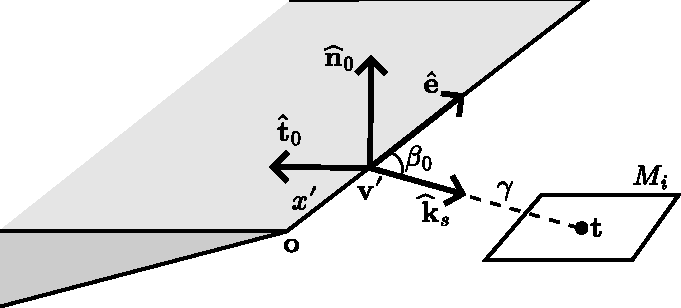
\includegraphics[width=\textwidth]{figures/radio-map-solver-diffraction-frame.pdf}
        \caption{3D view}
        \label{fig:radio-map-solver-diffraction-frame-3d}
    \end{subfigure}
    \hfill
    \begin{subfigure}[b]{0.40\textwidth}
        \centering
        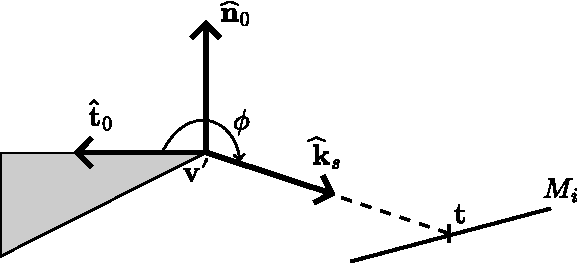
\includegraphics[width=\textwidth]{figures/radio-map-solver-diffraction-frame-2.pdf}
        \caption{2D cross-section}
        \label{fig:radio-map-solver-diffraction-frame-2d}
    \end{subfigure}
    \caption{
    A measurement point $\tv$ reachable by a diffracted ray from a wedge is determined by a distance along the edge $x'$ and the Keller cone azimuth $\phi$, while the cone opening angle is $\beta_0'$. 
    \label{fig:radio-map-solver-diffraction-frame}}
\end{figure}

With this reparametrization,~\eqref{eq:radio-map-solver-ci-D} becomes:
\begin{equation}
    \label{eq:radio-map-solver-ci-D-2}
    C_i^{(\Dc)} = \frac{1}{\abs{M_i}} \int_{0}^{L_{\Ec}} \int_{n\pi} \int_{0}^{L_{\Ec}} e \LB p \RB \Vc\LB p \RB w \LB p \RB \norm{ \frac{\delta \tv}{\delta x} \times \frac{\delta \tv}{\delta \phi} } dx d\phi dx'
\end{equation}
where $n\pi$ is the wedge exterior angle, and $\norm{ \frac{\delta \tv}{\delta x} \times \frac{\delta \tv}{\delta \phi} }$ accounts for the change of variables~\cite{Wikipedia_Surface_Integral}.

The condition in~\eqref{eq:radio-map-solver-ci-D-condition} is only satisfied when $x = x'$ for a given $\phi$, leading to:
\begin{equation}
    \label{eq:radio-map-solver-ci-D-3}
    C_i^{(\Dc)} = \frac{1}{\abs{M_i}} \int_{0}^{L_{\Ec}} \int_{n\pi} e \LB p \RB \Vc\LB p \RB \norm{ \frac{\delta \tv}{\delta x} \times \frac{\delta \tv}{\delta \phi} } dx d\phi.
\end{equation}

To estimate~\eqref{eq:radio-map-solver-ci-D-3}, $N_S'$ samples are drawn on the wedge: $x$ uniformly in $[0, L_{\Ec}]$ and $\phi$ uniformly in $[0, n\pi]$. This yields the Monte Carlo estimator:
\begin{equation}
    \label{eq:radio-map-solver-ci-D-est}
    \widehat{C}_i^{(\Dc)} = \frac{1}{\abs{M_i}} \frac{L_{\Ec}n\pi}{N_S'}\sum_{n=1}^{N_S'} e \LB p_n \RB \mathbb{I}\LB p_n \RB \norm{ \frac{\delta \tv}{\delta x} \times \frac{\delta \tv}{\delta \phi} }
\end{equation}
where $p_n$ is the $n$-th path, $\mathbb{I}\LB p_n \RB$ is 1 if $p_n$ intersects the measurement surface and is not occluded by other scatterers and 0 otherwise, and the weighting factor $\norm{ \frac{\delta \tv}{\delta x} \times \frac{\delta \tv}{\delta \phi} }$ is computed as described in Annex~\ref{sec:diffraction-radio-map-weighting-factor}.

\subsection{Non-Coherent vs. Coherent Radio Maps}

The proposed definition of radio maps involves a non-coherent summation of path gains~\eqref{eq:radio-map-solver-path-gain}. As a result, it does not capture fast fading effects, which result from the constructive and destructive interference of multiple paths. Figure~\ref{fig:radio-map-solver-fast-fading} demonstrates this by comparing three scenarios: a radio map generated using the radio map solver, a radio map created by non-coherently summing the path coefficients~\eqref{eq:path-coefficient} calculated with the path solver (Section~\ref{sec:path-solver}) by placing a single target at the center of each measurement cell, and a radio map produced by coherently summing the path coefficients~\eqref{eq:path-coefficient} calculated with the path solver, also by placing a single target at the center of each measurement cell. The radio map obtained using the radio map solver aligns with the non-coherent summation of path coefficients calculated using the path solver, as anticipated. However, it does not account for fast fading effects, which requires the coherent summation of path coefficients.

\begin{figure}[ht!]
    \centering
    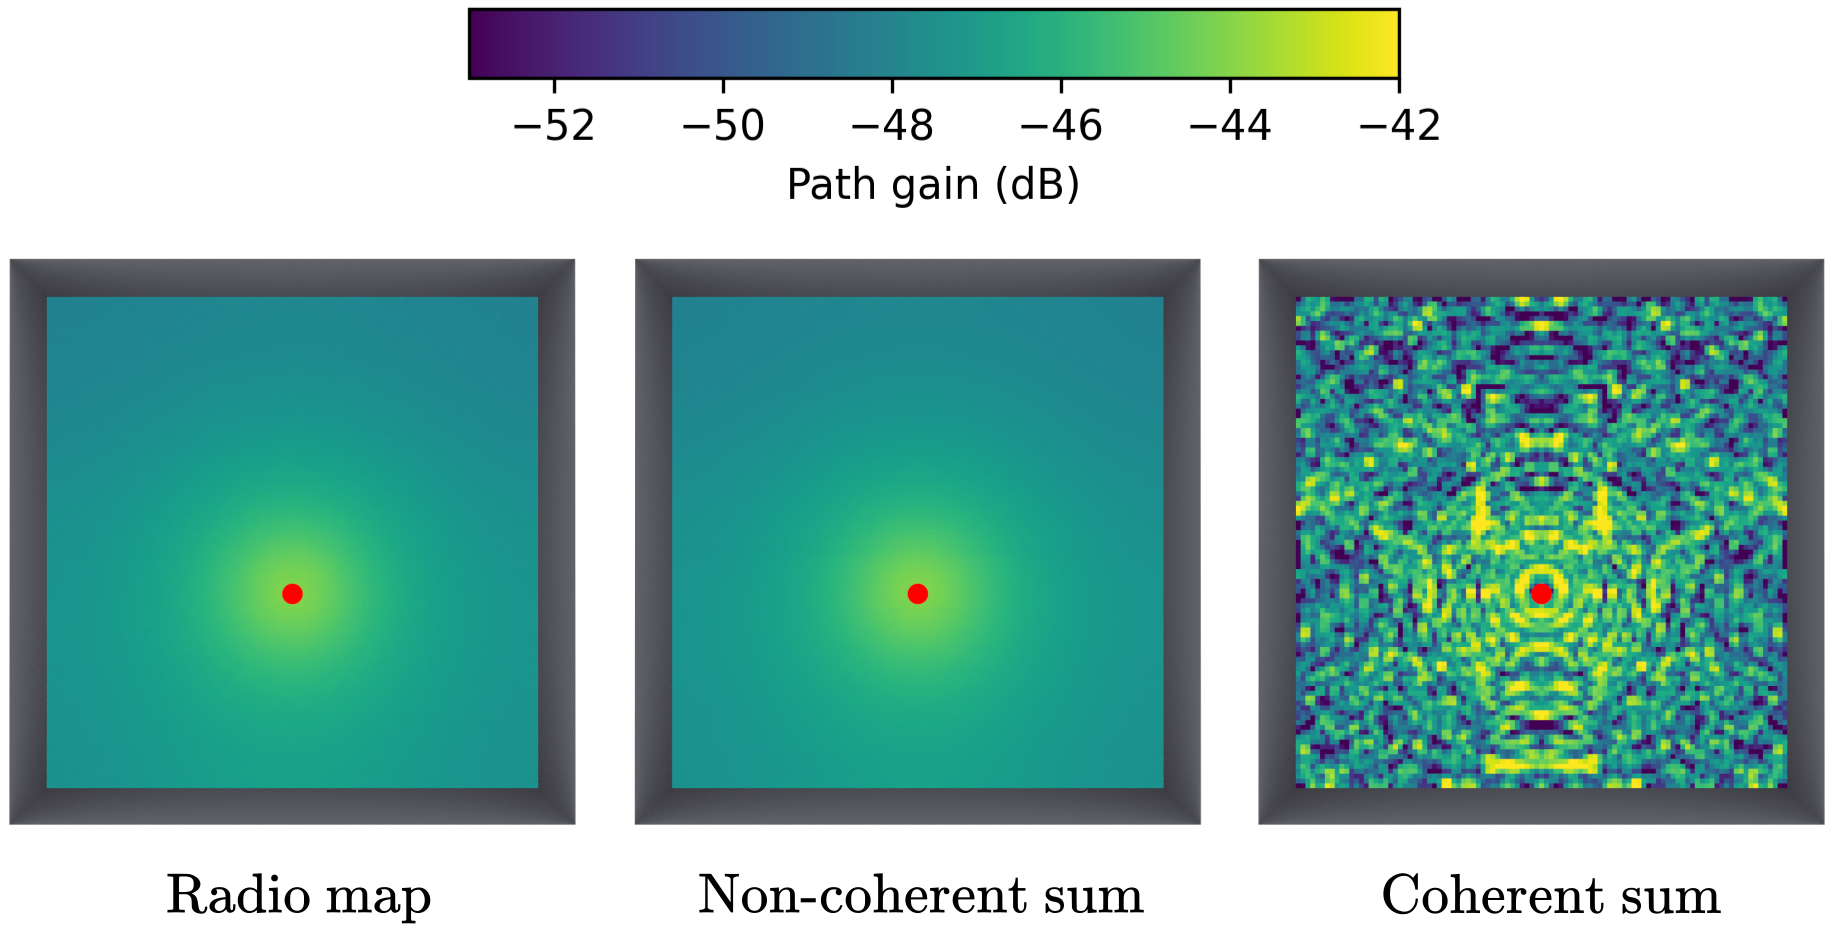
\includegraphics[width=0.75\textwidth]{figures/radio-map-solver-fast-fading.png}
    \caption{Comparison of radio maps: one computed using the radio map solver, one by non-coherently summing path coefficients from the path solver, and one by coherently summing path coefficients from the path solver. The transmitter is depicted as a red ball. All radio maps are computed with a maximum depth of $L = 3$, cell sizes of $10 \times 10$ cm, using isotropic antenna patterns on both the transmitter and receiver, and for the ``box'' scene built in \SRT{}. The ``non-coherent sum'' and ``coherent sum'' radio maps are generated by placing a single target point at the center of each measurement cell.\label{fig:radio-map-solver-fast-fading}}
\end{figure}

\subsection{Handling Multiple Transmit Antennas}
\label{sec:radio-map-solver-antenna-arrays}

The \SRT{} radio map solver supports antenna arrays of any size at the transmitter and allows for user-defined precoding vectors. However, it only supports synthetic arrays. In this setup, paths are generated from a single source located at the center of the array, and the channel response for each individual antenna is calculated by applying the appropriate phase shifts synthetically. This approximation holds true as long as the array size is small compared to the distance from the transmitter to the measurement plane and scatterers.

Using synthetic arrays enables efficient scaling with respect to the number of antennas. To see this, let $N_A^{\text{tx}}$ denote the number of antennas at the transmitter, and let $\uv_P \in \CC^{N_A^{\text{tx}}}$ be the precoding vector. For a given path connecting the source to the measurement plane, let $\Em \in \CC^2$ represent the electric field observed at the measurement plane. By employing a synthetic array, the corresponding electric fields for each antenna element are obtained by applying the array response vector~\eqref{eq:path-solver-array-response-vector}, denoted as $\uv_A^{\text{tx}}$, leading to
\begin{equation}
    \Em_A = \Em \LB \uv_A^{\text{tx}} \RB\tp.
\end{equation}
Here, $\Em_A$ is a matrix of size $2 \times N_A^{\text{tx}}$, where each column represents the electric fields radiated by each transmit antenna. The contribution of this path to the radio map is given by
\begin{equation}
    \norm{\Em_A \uv_P}^2.
\end{equation}
This expression allows the path's contribution to the radio map to be represented as
\begin{equation}
    \norm{\Em_A \uv_P}^2 = \norm{\LB \Em \LB \uv_A^{\text{tx}} \RB \tp \uv_P \RB}^2 = \norm{\Em \alpha}^2
\end{equation}
where $\alpha = \LB \uv_A^{\text{tx}} \RB\tp \uv_P$ is a scalar, which depends on the departure direction of the path from the transmitter and thus varies for paths originating from the source. By precomputing $\alpha$ for each path, the effect of the transmitter array can be efficiently simulated by multiplying the electric field of each path by $\alpha$ whenever the path intersects the measurement surface. This operation does not depend on the size of the array.

\begin{figure}[htbp]
    \centering
    \begin{subfigure}[b]{0.3\textwidth}
        \centering
        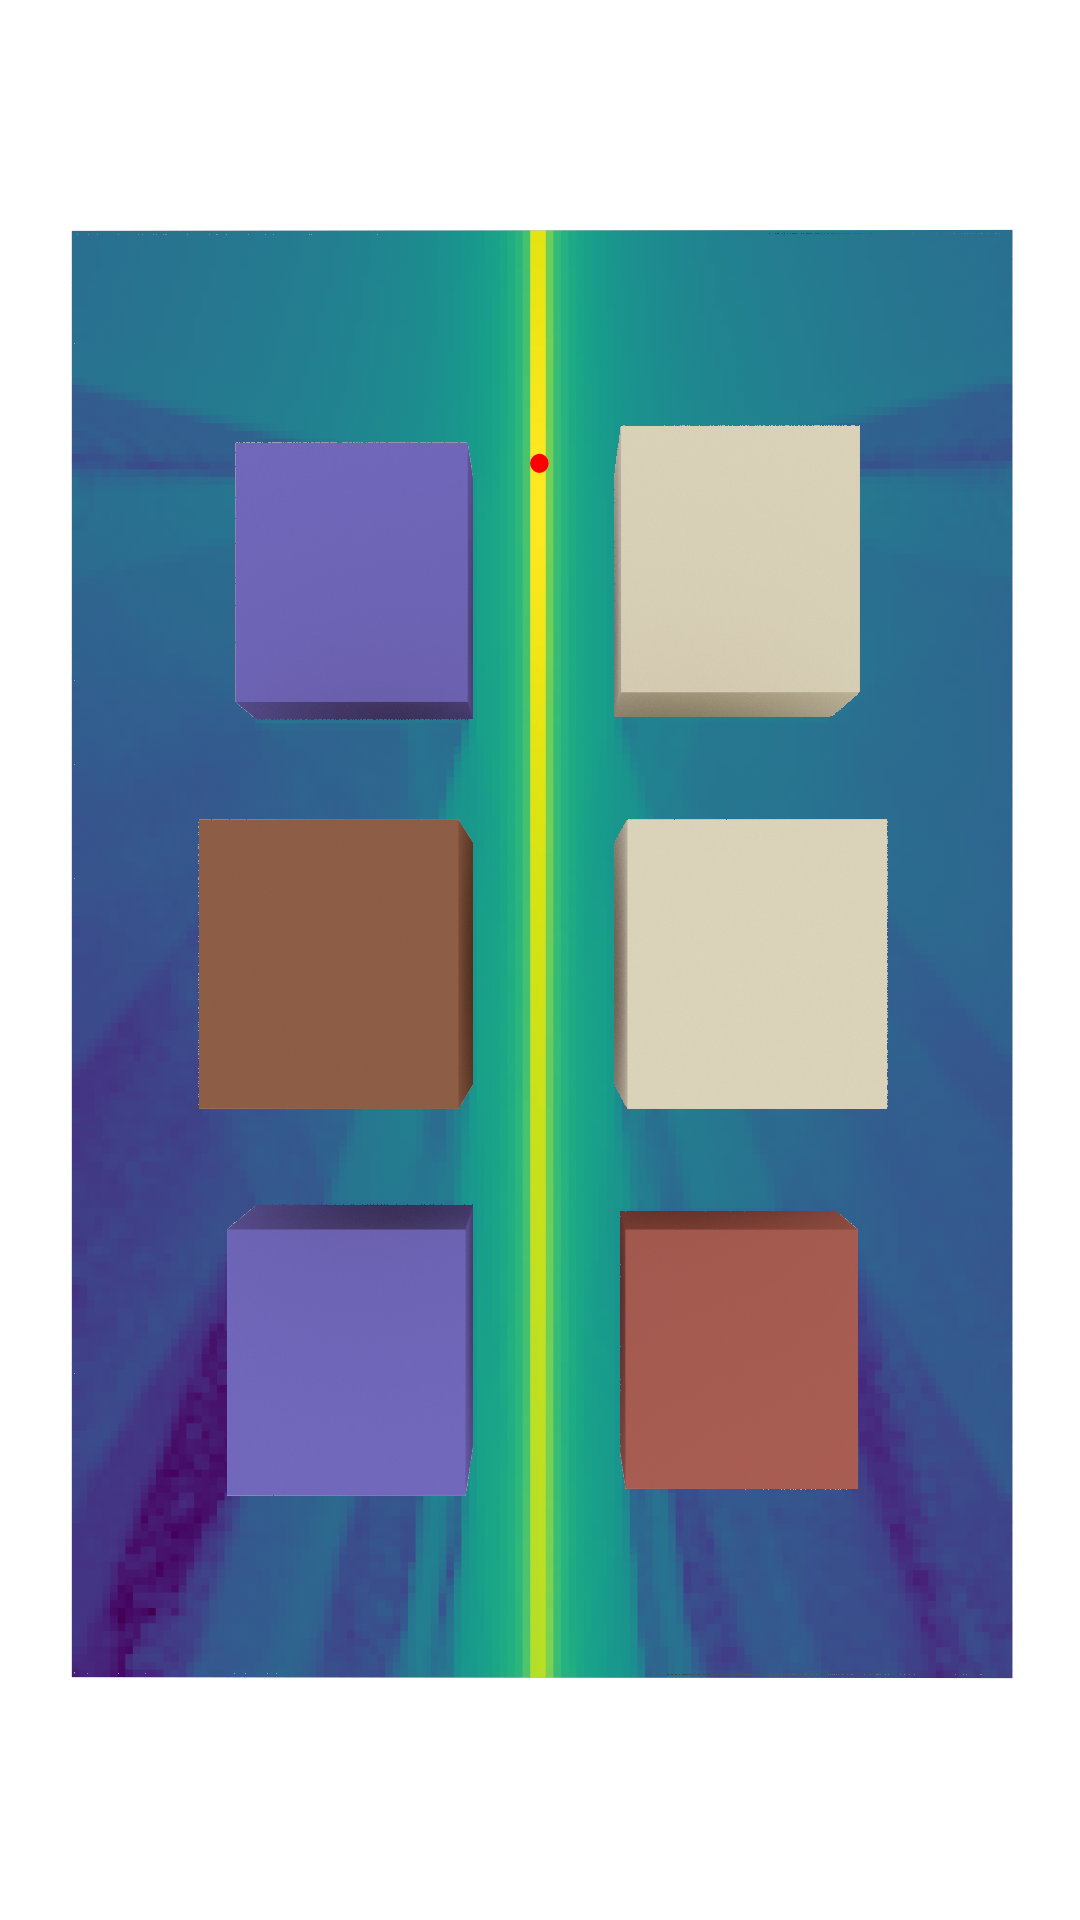
\includegraphics[width=\textwidth]{figures/radio-map-solver-sbr-scene.png}
        \caption{Scene with the radio map.\label{fig:radio-map-solver-sbr-scene}}
    \end{subfigure}
    \hfill
    \begin{subfigure}[b]{0.65\textwidth}
        \centering
        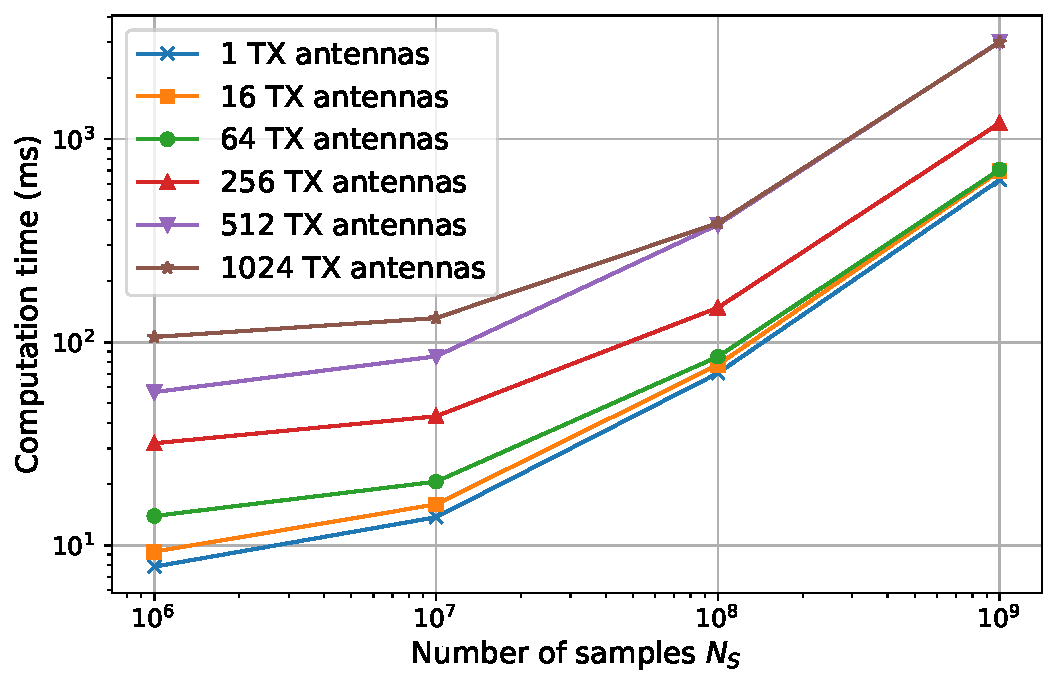
\includegraphics[width=\textwidth]{figures/radio-map-solver-sbr-scaling.pdf}
        \caption{Computation time vs. number of samples $N_S$.\label{fig:radio-map-solver-sbr-scaling}}
    \end{subfigure}
    \caption{Computation time for calculating radio maps using an NVIDIA RTX 4090 GPU for a single transmitter with a linear array of 1 to 1024 antennas.}
\end{figure}

Figure~\ref{fig:radio-map-solver-sbr-scaling} illustrates the computation time needed to generate a radio map for a single source as the number of samples $N_S$ and the number of transmit antennas $N_A^{\text{tx}}$ are varied. The setup, depicted in Figure~\ref{fig:radio-map-solver-sbr-scene}, employs the ``simple street canyon'' scene built into \SRT{}. The red ball indicates the source, positioned 20 meters above the ground. The radio map in Figure~\ref{fig:radio-map-solver-sbr-scene} is calculated using $10^8$ samples and a linear array of 512 transmit antennas. Notably, the radio map solver can compute radio maps with $10^9$ samples on a single NVIDIA RTX 4090 GPU.
The computation time increases with both the number of samples and antennas, exceeding one second only for the most demanding computations. It is important to note that while the computation time increases with the number of antennas due to the precomputation of the array weighting factor $\alpha$, it does not increase the memory usage of the radio map solver.

\paragraph{Handling of Dual-Polarized Transmit Antennas}

The radio map solver supports dual-polarized transmit antennas by considering two independent electric field vectors for each path. These are processed as if they were separate antenna elements (see Section~\ref{sec:radio-map-solver-antenna-arrays}).

\subsection{Practical Notes}

\paragraph{Mesh-based Measurement Surface}
\SRT{} supports mesh-based measurement surfaces, which are defined as collections of triangles (see Section~\ref{sec:essential-concepts-scene-objects-and-meshes}). In this case, each triangle serves as a measurement cell. Meshes can possess arbitrary topology, making this feature well suited for computing radio maps over complex terrains.

\paragraph{Scaling with the Number of Measurement Cells}
A key benefit of the radio map solver is that the compute required to generate the radio map remains constant regardless of the number of measurement cells. However, increasing the number of measurement cells will naturally require more memory for storage. Additionally, when the size of the measurement cells is reduced, it may be necessary to increase the number of samples $N_S$ to maintain the accuracy of the estimators~\eqref{eq:radio-map-solver-ci-all-2-estimator} and~\eqref{eq:radio-map-solver-ci-D-est}, as fewer paths will intersect with each measurement cell, resulting in noisier radio maps.

\paragraph{Early Termination with Russian Roulette and Gain Thresholding}
The radio map solver allows for early deactivation of paths using two techniques: Russian roulette and gain thresholding.
With gain thresholding, a path with ray tube length $r$ is deactivated when the squared amplitude of the electric field $\norm{\Em}^2$ falls below a user-defined threshold.
With Russian roulette, at each iteration, a path continues with a probability given by
\begin{equation}
    \label{eq:radio-map-solver-rr-prob}
    p_{\text{rr}} = \min\LB r^2 \norm{\Em}^2, p_{\text{rr,max}} \RB
\end{equation}
where $p_{\text{rr,max}}$ is the maximum probability, set by the user, for keeping the path active.
Both features can be enabled simultaneously and are applied only after a user-defined depth is reached.

\paragraph{Extension to other Types of Radio Maps}
The \SRT{} solver currently supports the calculation of channel gain maps, which are radio maps that provide an estimate of the channel gain for each cell. It is possible to extend the solver to calculate other types of radio maps, such as root-mean-square delay spread maps and angular spread maps~\cite{instant_rm}.
